\section{SignalGP}

% Broad overview of SignalGP
As with other tag-based systems, 
SignalGP agents (programs) are defined by a set of functions (modules) where each function is referred to using a tag and contains a linear sequence of instructions.
To augment this framework, SignalGP also makes explicit the concept of \textit{events} where event-specific data is associated with a tag that agents can use to specify how that event should be handled.  
In this work, we arbitrarily chose to represent tags as fixed-length bit strings. 
Agents may both generate internal events and be subjected to events generated by the environment or by other agents. 
Events trigger functions based on the similarity of their tags. When an event triggers a function, the function is run with the event's associated data as input. 
SignalGP agents handle many events simultaneously by processing them in parallel. 
Figure \ref{chapter:signalgp:fig:signalgp-overview} shows a high-level overview of SignalGP. 

\begin{figure*}[!ht]
  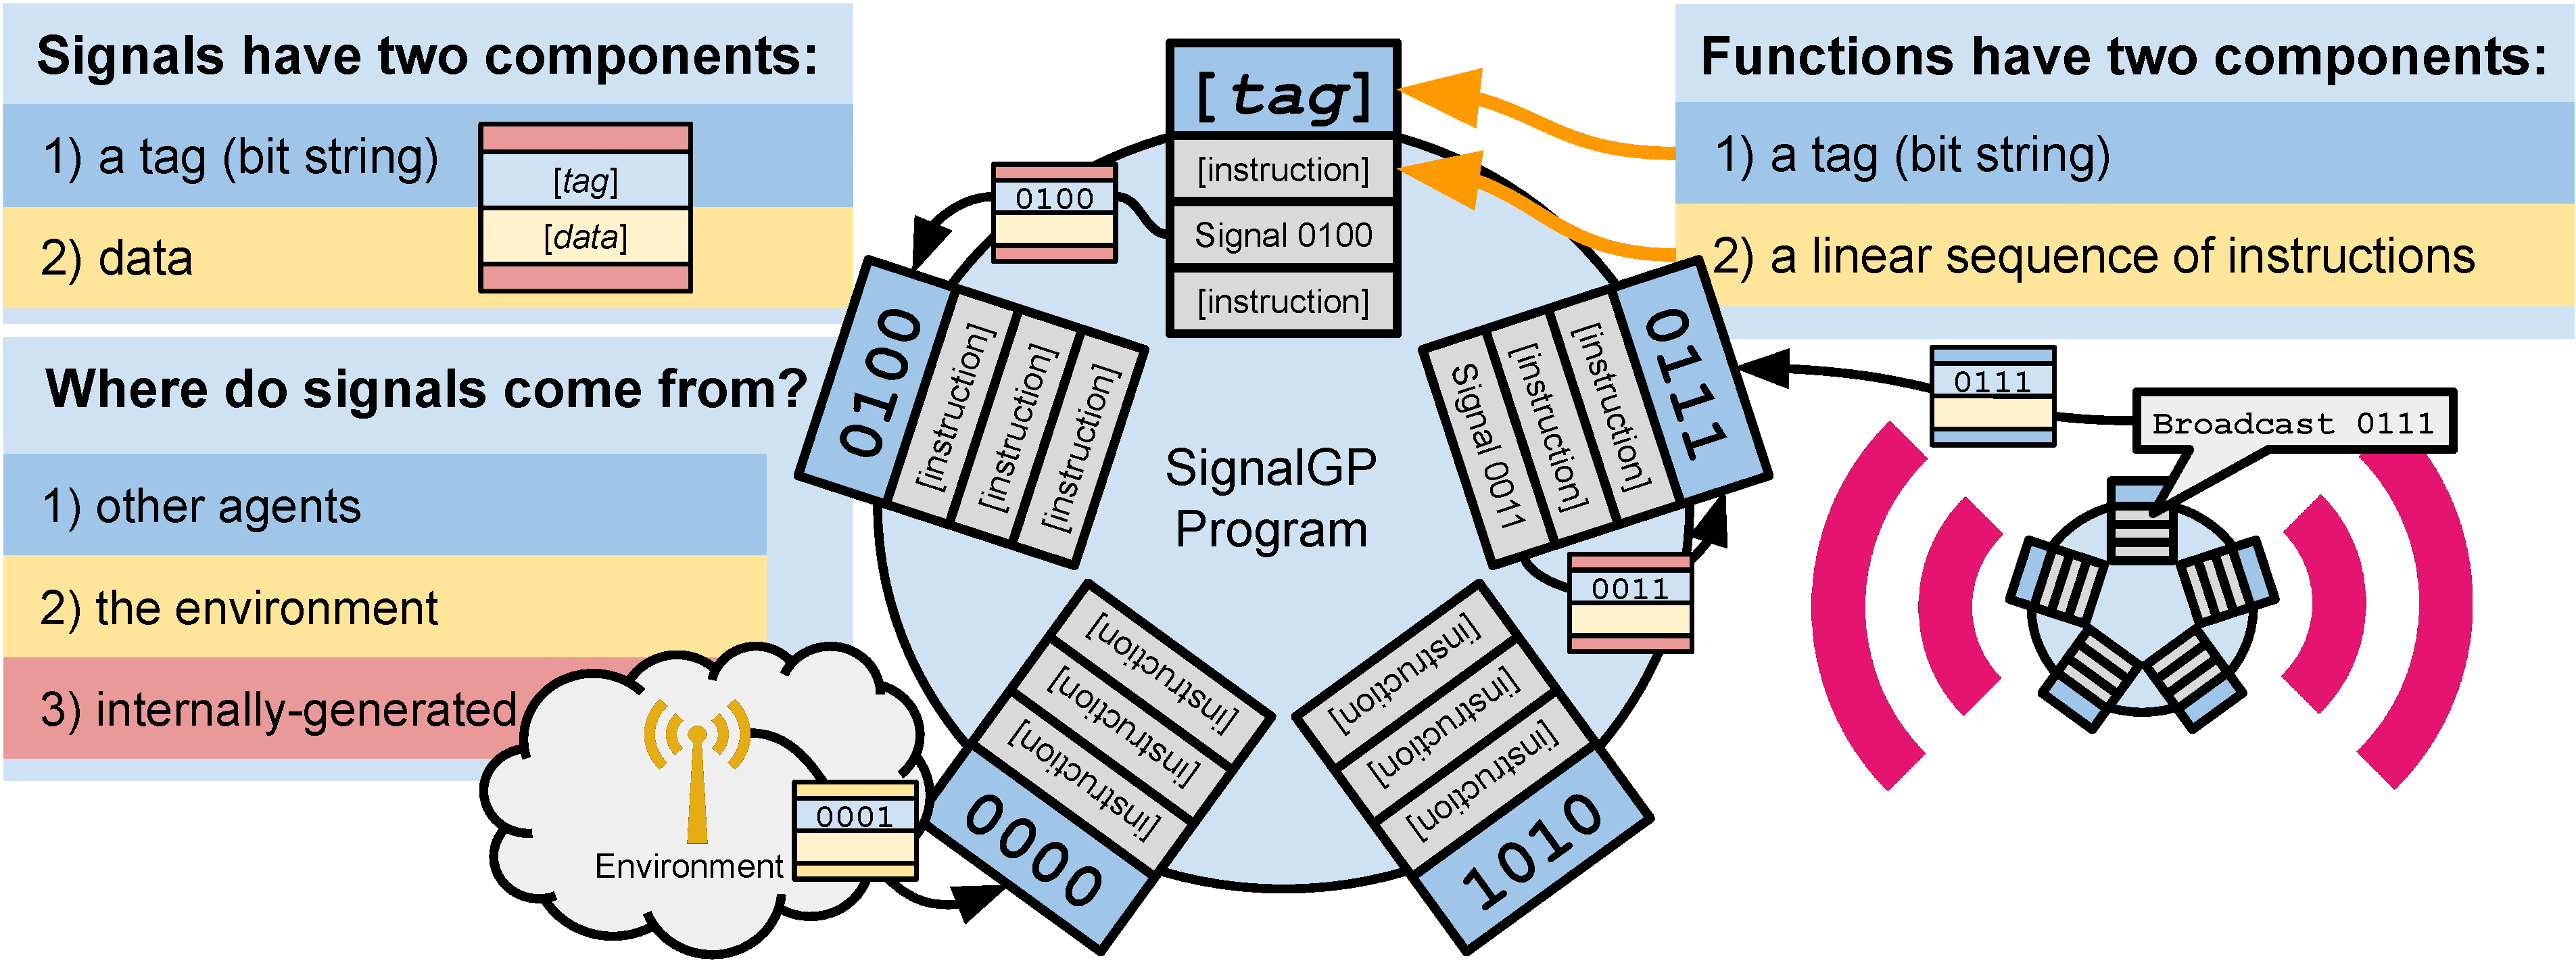
\includegraphics[width=\textwidth]
  {chapters/04-evolving-event-driven-programs-with-signalgp/media/signalgp-overview.pdf}
  \caption{\small 
  \textbf{A high-level overview of SignalGP.}
  SignalGP programs are defined by a set of functions.
  Events trigger functions with the \textit{closest matching} tag, allowing SignalGP agents to respond to signals. 
  SignalGP agents handle many events simultaneously by processing them in parallel.
  }
  \label{chapter:signalgp:fig:signalgp-overview}
\end{figure*}

\subsection{Tag-based Referencing}
\label{chapter:signalgp:sec:signalgp:tag-based-referencing}

Incorporating modules (\textit{e.g.}, functions, subroutines, macros, \textit{etc.}) into genetic programming has been extensively explored, and the benefits of modules in GP have been well documented
(\textit{e.g.}, \citep{koza_genetic_1992,koza_genetic_1994,angeline_evolutionary_1992,keijzer_undirected_2005,walker_automatic_2008,roberts_evolving_2001,spector_simultaneous_1996}). 
The main purpose of SignalGP functions are to act as event-handlers---computations triggered in response to signals. However, they have the additional benefit of providing explicit architectural support for program modularity, bestowing the boon of reusable code. 
As with any reusable code block in GP, the question remains: how should the code be referenced? 
The answer to this question can be reused to answer the following question: how should we determine which event-handlers are triggered by events? 

Inspired by John Holland's concept of a ``tag'' \citep{holland_effect_1993,holland_genetic_1987,holland_concerning_1990,holland_studying_2006} as a mechanism for matching, binding, and aggregation, Spector \textit{et al.} \citep{spector_tag-based_2011,spector_whats_2011,spector_tag-based_2012} introduced and demonstrated the value of tag-based referencing in the context of GP. 
In this context, a tag-based reference always links to a tagged entity with its closest match. 
These tagged entities include instructions and sequences of code (\textit{i.e.}, modules), providing an evolvable mechanism for code referencing. 

SignalGP shifts these ideas into a more fully event-driven context.
In SignalGP, sets of instructions are modularized into functions that are labeled with tags. Events are made explicit and trigger those functions with whose tags have the closest match.
The underlying instruction set is crafted to easily trigger internal events, broadcast external events, and to otherwise work in a tag-based context. 
Finally, SignalGP can be configured to only match tags that are relatively close (within a threshold) allowing agents to ignore events entirely by avoiding the use of similar tags.

\subsection{Virtual Hardware} 

As in many GP representations, linear GP programs are often interpreted in the context of virtual hardware, which typically comprises memory---usually in the form of registers or stacks---and other problem-specific virtual hardware elements, allowing programs to achieve complex functionality \citep{mcdermott_genetic_2015,poli_field_2008,ofria_avida:_2009}. 
SignalGP programs are interpreted by virtual hardware consisting of the following four major components: program memory, an event queue, a set of execution threads, and shared memory.

\textbf{Program memory} stores the SignalGP program currently executing on the virtual hardware.

The \textbf{event queue} manages recently received events waiting to be dispatched and processed by functions. The event queue dispatches events in the order they are received. 

The SignalGP virtual hardware supports an arbitrary number of \textbf{execution threads} that run concurrently. 
Each thread processes a single instruction every time step. 
In the same way that Byers \textit{et al.}'s parallel-executing digital enzymes \citep{byers_digital_2011} allow a robot controller to process many external stimuli simultaneously, parallel execution allows SignalGP agents to handle many events at once.

Each thread maintains a call stack that stores state information about the thread's active function calls. 
The current state for any given thread resides at the top of the thread's call stack. 
Call states maintain local state information for the function call they represent: a function pointer, an instruction pointer, input memory, working memory, and output memory. 
A function pointer indicates the current function being run. 
An instruction pointer indicates the current instruction within that function. 
Input, working, and output memory serve as local memory. 

Working memory is used for performing local operations (\textit{e.g.}, addition, subtraction, multiplication, \textit{etc.}). 
Input memory is analogous to function arguments (\textit{i.e.}, function input), and output memory is analogous to function return memory (\textit{i.e.}, what is returned when a function call concludes). 
By convention, instructions can both read from and write to working memory, input memory is read-only, and output memory is write-only. 
To use an analogy, working memory, input memory, and output memory are to SignalGP functions as hidden nodes, input nodes, and output nodes are to conventional artificial neural networks.  
\textbf{Shared memory} serves as global memory. 
Shared memory is accessible (\textit{i.e.}, readable and writable) by all threads, allowing them to store and share information. 

\subsection{Program Evaluation}

SignalGP programs are sets of functions where each function associates an evolvable tag with a linear sequence of instructions. 
In our implementation of SignalGP, instructions are argument-based, and in addition to evolvable arguments, each instruction has an evolvable tag. 
Arguments modify the effect of the instruction, often specifying memory locations or fixed values. 
Instruction tags may also modify the effect of an instruction. For example, instructions that refer to functions do so using tag-based referencing. 
Further, instructions use their tag when generating events, either to be broadcast to other SignalGP agents or to be handled internally for their own use. 

Program evaluation can be initialized either actively or passively.  
During active initialization, the program will begin evaluation by automatically calling a designated main function on a new thread.  
In passive initialization, computation takes place only in response to external events.  
In the work presented here, we use only active initialization and automatically reset the main thread if it would have otherwise terminated.

While executing, the SignalGP virtual hardware advances on each time step in three phases: 
(1) All events in the event queue are dispatched, with each triggering a function \textit{via} tag-based referencing. 
(2) Each thread processes a single instruction. 
(3) Any threads done processing are removed.
Phases occur serially and in order. 

Executed instructions may call functions, manipulate local and shared memory, generate events, perform basic computations, control execution flow, \textit{et cetera} (see supplementary material \citep{signalgp_supplement_2018} for details on all instructions used in this work).
Instructions in SignalGP are guaranteed to always be syntactically valid, but may be functionally useless. 
Every instruction has three associated arguments and an associated tag. 
Not all instructions make use of their three arguments or their tag; unused arguments and tags are not under direct selection and may drift until a mutation to the operand reveals them.

% \vspace{2mm}
% \noindent\textbf{Instruction-triggered Function Calls}\\
\subsubsection{Instruction-triggered Function Calls}

Functions in SignalGP may be triggered by either instruction calls or events.
When a \code{Call} is executed, the function in program memory with the most similar tag to the \code{Call} instruction's tag (above a similarity threshold) is triggered; in this work, ties are broken by a random draw (though any tie-breaking procedure could be used).  
Tag similarity is calculated as the proportion of matching bits between two bit strings (simple matching coefficient).  

When a function is triggered by a \code{Call} instruction, a new call state is created and pushed onto that thread's call stack.
The working memory of the caller state is copied as the input memory of the new call state (\textit{i.e.}, the arguments to the called function are the full contents of the previous working memory). 
The working memory and the output memory of the new call state are initially empty. 
To prevent unbounded recursion, we place limits on call stack depth; if a function call would cause the call stack to exceed its depth limit, the call instead behaves like a no-operation. 

Instruction-triggered functions may return by either executing a \code{Return} instruction or by reaching the end of the function's instruction sequence. 
When an instruction-triggered function returns, its call state is popped from its call stack, and anything stored in the output memory of the returning call state is copied to the working memory of the caller state (otherwise leaving the caller state's working memory unchanged). 
In this way, instruction-triggered function calls can be thought of as operations over the caller's working memory. 

% \vspace{2mm}
% \noindent\textbf{Event-triggered Function Calls}\\
\subsubsection{Event-triggered Function Calls}

Events in SignalGP are analogous to external function calls. 
When an event is dispatched from the event queue, the virtual hardware chooses the function with the highest tag similarity score (above a similarity threshold) to handle the event.
In this work, ties are broken by a random draw (though any tie-breaking procedure could be used). 

Once a function is selected to handle an event, it is called on a newly-created execution thread, initializing the thread's call stack with a new call state. 
The input memory of the new call state is populated with the event's data. 
In this way, events can pass information to the function that handles them. 
When the function has been processed (\textit{i.e.}, all of the active calls on the thread's call stack have returned), the thread is removed. 
To prevent unbounded parallelism, we place a limit on the allowed number of concurrently executing threads; if the creation of a new thread would cause the number of threads to exceed this limit, thread creation is prevented.

\subsection{Evolution}
\label{chapter:signalgp:sec:signalgp:evolution}

Evolution in SignalGP proceeds similarly to that of typical linear GP systems. 
Because function referencing is done \textit{via} tags, changes can be made to program architecture (\textit{e.g.}, inserting new or removing existing functions) while still guaranteeing syntactic correctness. 
Thus, modular program architectures can evolve dynamically through whole-function duplication and deletion operators or through function-level crossover techniques. 

In the studies presented in this paper, we evolve SignalGP programs directly (as opposed to using indirect program encodings), which requires SignalGP-aware mutation operators. 
We propagated SignalGP programs asexually and applied mutations to offspring. 
We used whole-function duplication and deletion operators (applied at a per-function rate of 0.05) to allow evolution to tune the number or functions in programs. 
We mutated tags for instructions and functions at a per-bit mutation rate (0.05). 
We applied instruction and argument substitutions at a per-instruction rate (0.005). 
Instruction sequences could be inserted or deleted via slip-mutation operators \citep{lalejini_gene_2017}, which facilitate the duplication or deletion of sequences of instructions; we applied slip-mutations at a per-function rate (0.05). 